%% BPFix: Rust-Style Diagnostics for eBPF Verifier Failures
%% Target: OSDI / SOSP / EuroSys (12 pages, anonymous review)
\documentclass[sigplan,10pt,anonymous,review]{acmart}

\usepackage{listings}
\usepackage{xcolor}
\usepackage{microtype}
\usepackage{graphicx}
\usepackage{booktabs}
\usepackage{multirow}
\usepackage{amsmath}
\usepackage{url}
\usepackage{subcaption}
\usepackage{tikz}
\usetikzlibrary{arrows.meta,positioning,shapes.geometric,fit}

\newcommand{\sys}{\textsc{BPFix}\xspace}
\usepackage{xspace}

%% Suppress acmart copyright block for draft
\setcopyright{none}
\acmDOI{}
\acmISBN{}
\acmConference[EuroSys '27]{ACM European Conference on Computer Systems}{April 2027}{Rotterdam, Netherlands}
\acmYear{2027}

%% Listings style for verifier output / C code
\lstdefinestyle{verifier}{
  basicstyle=\ttfamily\scriptsize,
  breaklines=true,
  columns=fullflexible,
  keepspaces=true,
  frame=none,
  aboveskip=2pt,
  belowskip=2pt,
}

\lstdefinestyle{bpfix}{
  basicstyle=\ttfamily\scriptsize,
  breaklines=true,
  columns=fullflexible,
  keepspaces=true,
  frame=none,
  aboveskip=2pt,
  belowskip=2pt,
  moredelim=[is][\bfseries\color{red!70!black}]{/*bold*/}{/*end*/},
}

\lstdefinestyle{ccode}{
  language=C,
  basicstyle=\ttfamily\scriptsize,
  keywordstyle=\bfseries,
  commentstyle=\itshape\color{gray},
  breaklines=true,
  columns=fullflexible,
  keepspaces=true,
  frame=none,
  aboveskip=2pt,
  belowskip=2pt,
  numbers=left,
  numberstyle=\tiny\color{gray},
  numbersep=5pt,
}

%% Theorem environments (acmart provides amsthm)
\newtheorem{definition}{Definition}
\newtheorem{theorem}{Theorem}
\newtheorem{proposition}{Proposition}

%% Tighter spacing for figures
\setlength{\floatsep}{4pt}
\setlength{\textfloatsep}{6pt}
\setlength{\intextsep}{4pt}

%% Suppress widow/orphan lines
\widowpenalty=10000
\clubpenalty=10000

%% Allow slight flexibility to prevent overfull hboxes from inline \texttt{} tokens
\emergencystretch=1.5em

%% Fix fancyhdr headheight warning
\setlength{\headheight}{18.5pt}
\addtolength{\topmargin}{-5.5pt}

\begin{document}

\title{\sys: Rust-Style Diagnostics for eBPF Verifier Failures}

\begin{CCSXML}
<ccs2012>
   <concept>
       <concept_id>10011007.10011006.10011008.10011024.10011025</concept_id>
       <concept_desc>Software and its engineering~Compilers</concept_desc>
       <concept_significance>500</concept_significance>
   </concept>
   <concept>
       <concept_id>10011007.10011006.10011073.10011074</concept_id>
       <concept_desc>Software and its engineering~Software verification and validation</concept_desc>
       <concept_significance>500</concept_significance>
   </concept>
   <concept>
       <concept_id>10010520.10010521.10010537.10010538</concept_id>
       <concept_desc>Computer systems organization~Operating systems</concept_desc>
       <concept_significance>300</concept_significance>
   </concept>
</ccs2012>
\end{CCSXML}
\ccsdesc[500]{Software and its engineering~Compilers}
\ccsdesc[500]{Software and its engineering~Software verification and validation}
\ccsdesc[300]{Computer systems organization~Operating systems}

\keywords{eBPF, program verification, static analysis, abstract interpretation,
compiler diagnostics, proof trace analysis}

\begin{abstract}
eBPF programs must pass a complex static verifier whose rejection messages
are notoriously opaque---developers receive verbose, thousand-line logs
pinpointing symptoms but obscuring the underlying cause.
Fixing these rejections requires understanding \emph{where} the safety
proof broke, not just \emph{that} it broke: the source code may contain the
intended safety argument while the verifier's abstract domain loses track of it
through LLVM's lowering.

We observe that the verifier's execution trace is a complete record of a
proof attempt---a sequence of per-instruction abstract states.  By analyzing
\emph{abstract state transitions} across this trace (bounds collapses, type
downgrades, provenance loss), \sys automatically locates where the safety
proof broke and why, without requiring knowledge of which specific safety
condition was checked.  The transition pattern itself classifies the failure:
a safety property never established indicates a source bug; one established
then lost indicates a compiler-induced lowering artifact.

\sys operates entirely in userspace and requires no kernel modifications.
\end{abstract}

\maketitle

%% ==============================
\section{Introduction}
\label{sec:intro}
%% ==============================

% --- Para 1: System scene + problem ---
eBPF is the foundation for critical kernel extensions powering security
enforcement (Cilium, Katran), performance tracing (bcc, bpftrace), and
networking infrastructure in production Linux deployments. Ensuring safety,
however, requires each eBPF program to pass a mandatory static verifier, an
abstract interpreter that rigorously checks all instructions before execution.
Unfortunately, when verification fails, developers confront overwhelmingly
verbose diagnostic logs often spanning thousands of lines. These logs reveal
only symptoms at rejection points, leaving the root cause---typically a safety
proof destroyed deep within compiler-generated instructions---buried hundreds
of lines earlier. Consequently, debugging verifier rejections has become the
single largest productivity bottleneck in eBPF development, as confirmed by a
recent Linux Foundation security audit~\cite{nccaudit2024} and extensive
developer frustration on Stack Overflow~\cite{deokar2024}.

% --- Para 2: Evidence + why existing fails ---
Verifier-related bug reports and workaround commits repeatedly show
proof-reshaping workarounds: the source code may be correct, but the verifier's
abstract domain cannot track the developer's safety argument through LLVM's
lowering.  These rejections are inherent to the verifier's design and cannot
be eliminated by better diagnostics alone---but fixing them correctly
requires knowing \emph{where} the safety proof broke, which current tools
cannot provide. We find that
existing solutions fundamentally misunderstand the structure embedded within
verification traces: current tools either rely on shallow regular expressions
applied only to the final rejection message~\cite{prettyverifier2025} or feed
entire raw logs to general-purpose language
models~\cite{kgent2024}, neither approach recognizing the verifier trace as a
structured safety proof attempt.
\label{sec:intro-gap}

% --- Para 3: Key insight ---
Our key insight is that the verifier's execution trace is a complete record of
a proof attempt---a sequence of per-instruction abstract states---and that
analyzing \emph{abstract state transitions} across this trace reveals where
and why the safety proof broke.  The error message identifies which safety
condition was checked (we call this the required proof, used as a focus
mechanism), but the core analysis is detecting the instruction whose abstract
state transition---bounds collapse, type downgrade, provenance loss---caused
the violation.  We call this the ``proof-loss point.''  Crucially, the
transition pattern itself classifies the failure: a safety property never
established in the trace indicates a source-level programming bug, while one
established then lost indicates a compiler-induced lowering artifact.

% --- Figure 1: motivating example ---
\begin{figure*}[t]
\begin{minipage}[t]{0.31\linewidth}
\textbf{Panel A: Source code}
\vspace{2pt}
\begin{lstlisting}[style=ccode, firstnumber=1]
int parse_ext(struct xdp_md *ctx) {
    void *data = (void*)(long)ctx->data;
    void *data_end = (void*)(long)ctx->data_end;
    if (data+sizeof(struct ext) > data_end)
        return XDP_DROP;         // bounds check
    struct ext *e = data;
    // reads guarded by line 3
    __u16 len = __bpf_htons(e->len); // byte-swap
    data += len;                 // REJECTED
    /* "unbounded min value" */
}
\end{lstlisting}
\end{minipage}%
\hfill
\begin{minipage}[t]{0.33\linewidth}
\textbf{Panel B: Raw verifier output (excerpt)}
\vspace{2pt}
\begin{lstlisting}[style=verifier]
22: R0_w=inv(id=0,umax=65280,
    var_off=(0x0; 0xff00))
    R6_w=inv(id=0,umax=255,
    var_off=(0x0; 0xff))
22: (4f) r0 |= r6
23: R0_w=inv(id=0)   <-- bounds GONE
...
math between pkt pointer and register
with unbounded min value is not allowed
\end{lstlisting}
\vspace{2pt}
\textit{Pretty Verifier output:}
\begin{lstlisting}[style=verifier]
"The value added to the packet pointer
 has an unbounded minimum. Consider
 adding `& 0xFFFF` to bound the value."
\end{lstlisting}
\end{minipage}%
\hfill
\begin{minipage}[t]{0.33\linewidth}
\textbf{Panel C: \sys output}
\vspace{2pt}
\begin{lstlisting}[style=verifier]
error[E005]: lowering_artifact
  -- parse_ext.c
  |
3 | if (data+sizeof(ext) > data_end)
  | ^^^^^^^^^^^^^^^^^^^^^^^^^^^^^^^^
  | proof established
  | R5: pkt(off=0) -> pkt(off=4,r=4)
  |
7 | __u16 len = __bpf_htons(e->len);
  | ^^^^^^^^^^^^^^^^^^^^^^^^^^^^^^^^
  | proof lost: OR destroys bounds
  | R0: scalar(umax=65280) -> scalar
  |
8 | data += len;
  | ^^^^^^^^^^^
  | rejected: pkt_ptr + unbounded
  |
  = note: LLVM lowers htons() to byte-load,
    shift, OR. Verifier cannot track OR result.
  = help: Add clamp: len &= 0xFFFF;
\end{lstlisting}
\end{minipage}
\caption{The motivating example: SO \#70750259.  \textbf{Panel A}: source
code with a correct bounds check at line 3.  \textbf{Panel B}: the verifier's
raw output (60+ lines, excerpt shown) and Pretty Verifier's single-line
response---both pointing at the symptom, not the cause.  \textbf{Panel C}:
{\sys}'s Rust-style multi-span output tracing abstract state transitions through three
source locations: proof established (line 3), proof lost (line 7, OR
instruction destroys bounds), rejected (line 8).}
\Description{Three-panel motivating example. Panel A: C source with bounds check.
Panel B: raw verifier output and Pretty Verifier single-line response.
Panel C: \sys Rust-style multi-span diagnostic with proof-established, proof-lost, and rejected labels.}
\label{fig:motivating}
\end{figure*}

% --- Para 4: System + results ---
Motivated by this insight, we design and implement \sys, a userspace diagnostic
engine that detects safety-relevant abstract state transitions across verifier
traces, traces their causal chains back to the root-cause instruction, and
provides concise, Rust-inspired diagnostics pinpointing exactly where and why
the safety proof broke.  Section~\ref{sec:eval} defines the methodology used to
evaluate reliability, proof reconstruction, localization, object correlation,
baseline comparison, and latency.

% --- Contributions ---
In summary, this paper makes three main contributions:
\begin{itemize}
  \item Identifies a structured, generalizable framework (abstract state
        transition analysis) that precisely pinpoints verifier root-cause
        failures and systematically classifies failure types
        (\S\ref{sec:required-proof-reconstruction}--\S\ref{sec:formal-foundation}).

  \item Designs and implements \sys, a fast userspace diagnostic tool
        leveraging this framework to deliver concise, actionable verifier
        diagnostics
        (\S\ref{sec:state-trace-parsing}--\ref{sec:formal-foundation}).

  \item Defines an evaluation methodology for measuring diagnostic reliability,
        required-proof reconstruction, localization quality, object-CFG
        correlation, baseline comparisons, and runtime overhead
        (\S\ref{sec:eval}).
\end{itemize}

%% ==============================
\section{Background}
%% ==============================

\subsection{The eBPF Verification Pipeline}

eBPF programs are written in C or Rust, compiled by LLVM to BPF bytecode, and
submitted to the kernel via the \texttt{bpf()} syscall.  The Linux verifier
runs before any program executes.  It performs a dataflow-style abstract
interpretation~\cite{cousot1977,gershuni2019simple}: it walks all execution
paths through the bytecode, maintaining per-register abstract state and
enforcing a set of safety properties at each instruction.  Programs that
violate any property are rejected.

The key architectural point is that there are three distinct reasoning levels:
\begin{itemize}
  \item \textbf{Source level.}  The programmer reasons about C/Rust values,
        bounds checks, null checks, and pointer lifetimes.
  \item \textbf{Compiler level.}  LLVM transforms source into BPF bytecode,
        potentially splitting, merging, or reordering computations.
  \item \textbf{Verifier level.}  The verifier reasons about BPF register
        abstract state: types, scalar bounds (\texttt{umin/umax},
        \texttt{smin/smax}), pointer offsets, packet ranges, and provenance IDs.
\end{itemize}
A proof that is valid at the source level can be lost at the verifier level if
LLVM's lowering produces register state that the verifier's abstract domain
cannot represent.  This is the root cause of lowering artifacts.

\subsection{Anatomy of a \texttt{LOG\_LEVEL2} Trace}
\label{sec:trace-anatomy}

When \texttt{log\_level=2} is set in \texttt{BPF\_PROG\_LOAD}, the verifier
emits a complete per-instruction trace interleaving per-register abstract state
(type, scalar bounds, pointer offset, packet range, provenance ID), BTF source
annotations~\cite{linuxbtf}, \texttt{mark\_precise} backtracking chains, and
control flow merge points.  A typical 50-instruction program produces
100--300 lines.  We detail the parsing of each element in~\S\ref{sec:state-trace-parsing}.


%% ==============================
\section{Design: The \sys Diagnostic Engine}
%% ==============================

\subsection{Architecture Overview}

\sys is a five-stage pipeline that transforms a raw \texttt{LOG\_LEVEL2}
verifier trace into a structured multi-span diagnostic.
Figure~\ref{fig:pipeline} shows the architecture.

\begin{figure}[t]
\centering
\begin{tikzpicture}[
  stagebox/.style={rectangle, draw, rounded corners, minimum width=2.6cm, minimum height=0.5cm, align=center, font=\small},
  arr/.style={-Latex, thick},
  outbox/.style={rectangle, draw=gray, dashed, rounded corners, minimum width=2.6cm, text width=2.6cm, minimum height=0.4cm, align=center, font=\scriptsize\itshape},
  node distance=0.32cm and 1.0cm
]
  \node[stagebox] (log)    {1. Log Parser};
  \node[stagebox, below=of log] (trace)  {2. State Trace Parser};
  \node[stagebox, below=of trace] (proof) {3. Proof Engine};
  \node[stagebox, below=of proof] (btf)   {4. Source Correlator};
  \node[stagebox, below=of btf]   (rend)  {5. Diagnostic Renderer};

  \node[outbox, right=of log]   (e1) {error\_id, taxonomy class};
  \node[outbox, right=of trace] (e2) {per-insn reg state\\BTF maps, backtracks};
  \node[outbox, right=of proof] (e3) {state transitions\\transition witnesses\\proof lifecycle labels};
  \node[outbox, right=of btf]   (e4) {BTF source spans\\with proof roles};
  \node[outbox, right=of rend]  (e5) {Rust-style text + JSON};

  \draw[arr] (log) -- (trace);
  \draw[arr] (trace) -- (proof);
  \draw[arr] (proof) -- (btf);
  \draw[arr] (btf) -- (rend);
  \draw[arr] (log) -- (e1);
  \draw[arr] (trace) -- (e2);
  \draw[arr] (proof) -- (e3);
  \draw[arr] (btf) -- (e4);
  \draw[arr] (rend) -- (e5);

  \node[above=0.3cm of log, font=\small\bfseries] {Verifier LOG\_LEVEL2 trace};
\end{tikzpicture}
\caption{\sys five-stage pipeline.  \texttt{bpfix} owns the diagnostic product
layer, while \texttt{bpfanalysis} provides verifier-log and BPF bytecode
analysis facts.}
\Description{Five-stage pipeline diagram: Log Parser, State Trace Parser, Proof Engine, Source Correlator, Diagnostic Renderer, each with labeled output boxes showing intermediate results.}
\label{fig:pipeline}
\end{figure}

Each stage is independently testable and produces a well-defined intermediate
representation.

\subsection{State Trace Parsing}
\label{sec:state-trace-parsing}

The log parser (Stage 1) handles error message identification: it matches
the final error line against error patterns and maps each pattern to
a taxonomy class (\textit{source\_bug}, \textit{lowering\_artifact},
\textit{verifier\_limit}, \textit{env\_mismatch}, \textit{verifier\_bug}).

The state trace parser (Stage 2) parses the remaining structure.  For each
BPF instruction, it extracts:
\begin{itemize}
  \item Instruction index, opcode, and mnemonic
  \item Pre/post-state per live register (type, \texttt{umin/umax},
        \texttt{smin/smax}, offset, packet range, provenance ID)
  \item BTF source annotation (file, line, column) if present
  \item Backtracking links from \texttt{mark\_precise} annotations
  \item Branch merge points with state at each join
\end{itemize}

The primary challenge is format variability.  Register state can appear before
or after the instruction, in branch merge lines, in backtracking annotations,
or across multiple lines.  The parser normalizes all variants into a uniform
\texttt{TracedInstruction} representation.

\textbf{Backtracking chain extraction.}  The verifier's own
\texttt{mark\_precise} backward pass is emitted in the log as
\texttt{regs=R stack=S before K: (op)~...} annotations.  \sys extracts
these into a \texttt{BacktrackChain} structure: a sequence of
(instruction\_index, registers\_tracked) pairs.  This is the verifier's own
root-cause chain, expressed as debug text.

\subsection{Required-Proof Reconstruction}
\label{sec:required-proof-reconstruction}

The verifier trace contains thousands of abstract state transitions per
execution path; analyzing all of them would produce noise.  The required proof
serves as a \emph{focus mechanism}: given the error message and
the register state at the rejection point, \sys infers which safety
condition the verifier needed---the \emph{required proof}---expressed
as a formal predicate over register state.  This predicate then directs
the state-transition analysis in Section~3.4 to the relevant registers
and state dimensions.

\sys supports the verifier proof families shown in
Table~\ref{tab:proof-families}.
The error message identifies the proof \emph{family}.  The register state
at the rejection point provides concrete parameters.  \sys instantiates the
predicate template with these parameters.

\begin{table}[t]
  \centering
  \footnotesize
  \caption{Verifier proof families reconstructed by \sys.}
  \label{tab:proof-families}
  \resizebox{\columnwidth}{!}{%
  \begin{tabular}{llp{2.6cm}}
    \toprule
    \textbf{Family} & \textbf{Predicate} & \textbf{Example error} \\
    \midrule
    \texttt{packet\_access}     & \texttt{type==pkt \&\& off+sz<=r}      & invalid access to packet \\
    \texttt{map\_value\_bounds} & \texttt{0<=off \&\& off+sz<=val\_sz}   & invalid map value access \\
    \texttt{null\_check}        & \texttt{type!=*\_or\_null}              & map\_value\_or\_null deref \\
    \texttt{stack\_access}      & \texttt{fp\_off within frame bounds}   & invalid indirect read \\
    \texttt{helper\_arg\_type}  & \texttt{type==expected\_arg\_type}     & R1 scalar expected pkt \\
    \texttt{scalar\_bounds}     & \texttt{smin>=0 \&\& umax<=limit}      & unbounded min value \\
    \texttt{reference\_release} & \texttt{all refs released before exit} & Unreleased reference id=N \\
    \texttt{context\_access}    & \texttt{off+sz<=ctx\_size}             & invalid bpf\_context access \\
    \texttt{alignment}          & \texttt{off \% align == 0}             & misaligned access \\
    \texttt{type\_safety}       & \texttt{type matches expected}         & R1 inv expected fp \\
    \bottomrule
  \end{tabular}%
  }
\end{table}

This predicate instantiation is not pattern matching on error text.  The same
error message (\texttt{invalid access to packet}) with different register
states at the rejection point produces different predicate instances with
different parameters.  The predicate is grounded in the verifier's type system:
for packet access, the verifier literally checks
\texttt{reg.off~+~access\_size~<=~reg.range}; \sys infers this from the
register fields at the rejection point.

\textbf{Inference algorithm.}  For each error ID, \sys defines:
(1) which register(s) contain the failing object (extracted from the rejection
line), (2) which predicate template applies (from the proof family), and
(3) how to extract concrete parameters from the register state dump.  The
resulting predicate is a boolean function over register state that can be
evaluated at any point in the trace.

\subsection{Abstract State Transition Detection}

The core of \sys is detecting \emph{safety-relevant abstract state transitions}
across the verifier's execution trace.  Given the instantiated predicate $P$
from Section~\ref{sec:required-proof-reconstruction} as a focus mechanism, \sys
evaluates $P$ against the abstract state at every instruction, producing a
status sequence:
\[
  \underbrace{?, \ldots, ?}_{\text{unknown}},
  \underbrace{\top, \ldots, \top}_{\text{satisfied}},
  \underbrace{\bot, \ldots, \bot}_{\text{violated}}
\]

Each transition in this sequence corresponds to a concrete abstract state
change (e.g., a bounds collapse, type downgrade, or provenance loss) at a
specific instruction.  \sys labels each transition:
\begin{itemize}
  \item \emph{proof\_established}: the abstract state transition where $P$ becomes
        satisfied (\texttt{?} $\to$ \texttt{true})---e.g., a bounds check
        narrows a register's range
  \item \emph{proof\_holds}: instructions where the abstract state preserves $P$
  \item \emph{proof\_lost}: the abstract state transition where $P$ goes from
        satisfied to violated (\texttt{true} $\to$ \texttt{false})---the
        \emph{transition witness}, e.g., an OR instruction collapses bounds
  \item \emph{rejected}: the final error instruction (always identified)
\end{itemize}

If $P$ is never satisfied, the status is \textit{never\_established} (a source
bug: the required abstract state was never produced, indicating a missing safety
check).
If $P$ is satisfied but a subsequent state transition destroys it before the
rejection, the status is \textit{established\_then\_lost} (a lowering artifact:
the source has a valid check but compiler-generated instructions produce an
abstract state transition that the verifier's domain cannot track).

\textbf{Key distinction from heuristic approaches.}  The transition witness is
not ``detect a bounds collapse pattern.''  It is ``evaluate the specific
safety predicate at each abstract state and find the exact instruction whose
state transition broke it.''  Different predicates identify different
transition witnesses on the same trace.  This is formally grounded in the
verifier's abstract domain, not in ad hoc pattern detection.

\textbf{Register value lineage.}  Predicates reference registers, but register
names are reused across the trace.  A value computed in R0 may be copied to R3
before the access.  \sys tracks value identity across register moves and
copies.  If R3 is defined as a copy of R0 (\texttt{r3 = r0}), and the
proof predicate references the packet range of R0, \sys continues
tracking the range on R3 for subsequent instructions.  This register value
lineage is essential for correctly identifying proof-established and proof-lost
events across LLVM's register allocation.

\textbf{Proof propagation analysis.}  For lowering artifact detection, \sys
additionally checks whether the proof established at the bounds-check site
\emph{propagates} to the register used at the access site.  If a different
register is used for the access than the one whose range was established at
the check (a common LLVM pattern), \sys classifies this as a lowering
artifact regardless of whether the proof predicate was technically satisfied
at some earlier instruction.

\subsection{Formal Foundation: Abstract State Transition Analysis}
\label{sec:formal-foundation}

The state transition detection described above can be understood as a
\emph{second-order abstract interpretation}: \sys applies abstract
interpretation to the \emph{output} of another abstract
interpreter~\cite{cousot1977}.  This section formalizes the framework,
which applies to any abstract interpreter that emits per-step states.

\subsubsection*{Two layers of abstract interpretation}

\textbf{Layer 1} is the eBPF verifier itself.  Its input is BPF
bytecode; its abstract domain $D_1$ consists of register types, scalar
bounds $[\texttt{umin},\texttt{umax}]$, pointer offsets, and packet ranges.
Its output is a trace $T = (s_0, s_1, \ldots, s_n)$ where each $s_i \in D_1$
is the abstract state after the $i$-th instruction.

\textbf{Layer 2} is \sys.  Its input is the trace $T$; it analyzes
abstract state transitions $(s_{i-1}, s_i)$ at each step, focused by a
safety predicate $P$, and outputs a sequence of proof lifecycle labels
that identify where and how the proof broke.

\begin{definition}[Proof status lattice]
\label{def:lattice}
The proof status lattice is
$\mathcal{L} = \{\bot, \mathit{unknown}, \mathit{satisfied}, \mathit{violated}\}$
with ordering
$\bot \sqsubseteq \mathit{unknown} \sqsubseteq \mathit{satisfied}$
and
$\bot \sqsubseteq \mathit{unknown} \sqsubseteq \mathit{violated}$,
where $\mathit{satisfied}$ and $\mathit{violated}$ are incomparable.
The bottom element~$\bot$ represents an uninitialized status
(relevant registers not yet present in the abstract state);
$\mathit{unknown}$ represents a state where the predicate is evaluable but the
relevant registers are not yet constrained.  Each transition between lattice
elements corresponds to a safety-relevant abstract state transition in the
verifier trace.
\end{definition}

\begin{definition}[State transition transfer function]
\label{def:transfer}
Let $P : D_1 \to \{\mathit{true}, \mathit{false}, \mathit{unknown}\}$ be the
safety predicate instantiated from the rejection point
(\S\ref{sec:required-proof-reconstruction}).
For each traced instruction~$i$ with verifier state $s_i \in D_1$,
the transfer function $\tau_i : \mathcal{L} \to \mathcal{L}$ maps the
previous proof status to the status after observing the abstract state
transition at instruction~$i$:
\[
\tau_i(\ell) = \begin{cases}
  \mathit{sat} & P(s_i) \land \ell \in \{\mathit{unk}, \mathit{sat}\} \\[2pt]
  \mathit{vio} & \neg P(s_i) \land \ell = \mathit{sat} \\[2pt]
  \ell         & \text{otherwise}
\end{cases}
\]
\end{definition}

\noindent
The status sequence is computed by forward iteration:
$\ell_0 = \mathit{unknown}$,\;
$\ell_i = \tau_i(\ell_{i-1})$.

\begin{definition}[Transition witness]
\label{def:witness}
The transition witness is the smallest index $w$ such that
$\ell_{w-1} = \mathit{satisfied}$ and $\tau_w(\ell_{w-1}) = \mathit{violated}$.
This is the exact instruction where the proof breaks.
If no such $w$ exists and $\ell_n = \mathit{violated}$, the proof was
\emph{never established}.
\end{definition}

\begin{theorem}[Required-proof lifecycle soundness]
\label{thm:required-proof-soundness}
Assume the terminal rejection is mapped to the correct required proof~$P$, and
the monitor for~$P$ is sound with respect to the verifier check it represents:
when the monitor reports \textit{satisfied} at abstract state~$s_i$, every
concrete state $c \in \gamma(s_i)$ satisfies the checked safety condition, and
when it reports \textit{violated}, the verifier lacks the abstract evidence
needed to discharge that check at~$i$.  Then every lifecycle label emitted by
\sys corresponds to a real change in the verifier's abstract evidence for~$P$:
\textit{proof\_established} marks a transition from missing to established
evidence, \textit{proof\_lost} marks a transition from established to missing or
insufficient evidence, and \textit{rejected} marks a final state that does not
discharge~$P$.
\end{theorem}
\begin{proof}[Proof sketch]
The verifier is a sound abstract interpreter: each $s_i$ over-approximates all
concrete states reachable at instruction~$i$~\cite{gershuni2019simple}.  The
required-proof monitor maps each $s_i$ to the proof-status lattice by the
per-family predicate for~$P$.  By the monitor-soundness assumption, each
per-state status is a sound statement about the verifier's available evidence
for the corresponding check.  The lifecycle labels are emitted exactly at the
status transitions computed by the transfer function~$\tau_i$.  Therefore the
labels identify real changes in verifier abstract evidence for~$P$, though they
do not by themselves prove semantic root cause or repair correctness.
\end{proof}

\textbf{Proof-relevant backward slice.}
Given the transition witness $w$, the \emph{proof-relevant backward slice} is
\[
  S = \{ i < w \mid \exists\, r \in \mathit{regs}(P) .\;
    \text{instruction } i \text{ writes to } r \}
\]
i.e., all instructions before $w$ that write to registers appearing in the
proof predicate~$P$.  When \texttt{mark\_precise} backtracking
information is available in the trace, $S$ is refined to include only
instructions on the backtracking chain, yielding a tighter slice.

\textbf{Generalization beyond eBPF.}
Abstract state transition analysis applies to any abstract interpreter that
outputs per-step abstract states.  The requirements are:
(1)~per-step abstract states are emitted,
(2)~safety properties are expressible as predicates over the abstract domain,
and (3)~the trace is ordered.
The key insight is domain-independent: given a sequence of abstract states
$[s_0, \ldots, s_n]$ and a safety predicate~$P$, detecting the transition
$(s_{w-1}, s_w)$ where $P$ changes from satisfied to violated locates the
proof-loss point regardless of what the abstract domain represents.
Rust's borrow checker (lifetime predicates over borrow state), WebAssembly
validators (type predicates over operand stack state), and Java bytecode
verifiers (type predicates over stack frame state) all satisfy these
requirements---suggesting that abstract state transition analysis is a
general technique for improving diagnostic quality in verified language
runtimes.

\subsection{BTF Source Correlation}

\sys maps each detected state transition event (proof established, proof lost,
rejected) to its source location via BTF \texttt{line\_info}
annotations~\cite{linuxbtf}.
When the verifier emits a source-location comment before an instruction (e.g.,
\texttt{; foo.c:42}), \sys records the mapping.  Multiple consecutive bytecode
instructions from the same source line are merged into a single span.

When BTF annotations are absent, \sys falls back to bytecode-level spans
(instruction indices only).  Object files are optional enrichments: when an
object path is available, \texttt{bpfanalysis} can decode BPF instruction
sections, build \texttt{ProgramCFG} summaries, and attach verifier states to CFG
sites when the verifier PC layout matches the object section layout.

\subsection{Diagnostic Rendering}

\sys produces two output formats from the same state transition analysis:

\textbf{Human-readable Rust-style output.}  Modeled on Rust compiler
diagnostics~\cite{rustdiag2016}, the output shows multiple source spans
with causal labels, register state changes at each transition, and
\texttt{note}/\texttt{help} annotations.  The format is designed to be
readable in a terminal, an IDE, or a CI log without any tool support.

\textbf{Structured JSON.}  A machine-readable format containing
\texttt{error\_id}, \texttt{taxonomy\_class}, \texttt{proof\_status}, an array
of \texttt{spans} (each with role, source location, instruction index, and
state change), the instantiated proof predicate, and \texttt{note}/\texttt{help}
text.  This format is designed for consumption by LLM agents (replacing raw
log text in prompts), CI systems (structured failure annotations), and IDE
plugins.

\subsection{Implementation Notes}

\sys is implemented as a Rust Cargo workspace.  The \texttt{bpfix} crate owns
the command-line interface, required-proof reconstruction, user-facing failure
classes, text rendering, and JSON rendering.  The \texttt{bpfanalysis} crate
owns neutral facts: verifier-log state parsing, BPF instruction modeling,
bytecode lifting, \texttt{ProgramCFG} summaries, and verifier-state attachment.

\textbf{Log-first operation.}  \sys requires only verifier log text for its
basic diagnostic path.  Object files, source files, and external debug
information are optional enrichments.  This matches the intended workflow:
developers keep their current loader or build system and pass the captured
verifier log to \texttt{bpfix}.

\textbf{Language independence.}  Because \sys analyzes verifier logs and BPF
bytecode-level facts, it is agnostic to whether the original program was
written in C, Rust, Go, or another language.  The methodology in
Section~\ref{sec:eval} can stratify diagnostics by source language when
benchmark metadata records it.

%% ==============================
\section{Evaluation Methodology}
\label{sec:eval}
%% ==============================

We evaluate \sys on the versioned \texttt{bpfix-bench} corpus.  The benchmark
manifest is the case registry: each admitted case identifies a verifier log and,
when available, source metadata or an object file.  Runtime diagnosis consumes
only the verifier log and optional object path.  Benchmark labels are used after
diagnosis as evaluation oracles, not as inputs to the tool.

The evaluation is organized around six questions:
\begin{itemize}
  \item[\textbf{Q1}] Does \sys generate diagnostics reliably over admitted
        benchmark logs?
  \item[\textbf{Q2}] Which verifier proof families can \sys reconstruct, and
        which terminal rejections remain unknown?
  \item[\textbf{Q3}] Do emitted lifecycle spans identify useful source or
        bytecode locations for the rejected verifier proof?
  \item[\textbf{Q4}] How much does optional object-CFG correlation add
        beyond log-only diagnostics?
  \item[\textbf{Q5}] How does \sys compare with final-line and Pretty Verifier
        baselines on the same admitted corpus?
  \item[\textbf{Q6}] What is the runtime overhead of log-only and object-enriched
        diagnosis?
\end{itemize}

\subsection{Corpus}
\label{sec:corpus}

\texttt{bpfix-bench/manifest.yaml} is the canonical discovery entry point for
the corpus.  The corpus contains replayable verifier-failure cases from kernel
selftests, Stack Overflow questions, GitHub issues, and GitHub commits.  A case
is admitted when its manifest entry points to a readable verifier log and the
log contains a terminal verifier rejection.  Optional fields may provide source
files, object files, expected error annotations, fix locations, or language
metadata; these fields are used only for stratified analysis and scoring.

\subsection{Metrics}
\label{sec:metrics}

\textbf{Reliability.}  We measure whether \sys exits successfully and emits a
structured diagnostic for each admitted case.  Parser failures, object-analysis
failures, and unknown terminal rejections are reported separately so that
log-only diagnosis is not conflated with optional enrichment.

\textbf{Required-proof reconstruction.}  We classify each diagnostic by the
proof family in Table~\ref{tab:proof-families}.  The metric records whether a
known family was reconstructed, whether the terminal rejection fell into an
unknown family, and whether the rejection was outside verifier-proof diagnosis
scope.

\textbf{Localization quality.}  For cases with source, bytecode, or expected
error annotations, we compare \sys spans against the benchmark oracle.  The
primary spans are the rejected instruction, the proof-established site, and the
proof-lost site when such lifecycle events exist in the trace.

\textbf{Object correlation.}  For cases with object files, we run both log-only
and object-enriched diagnosis.  The object-enriched run measures whether BPF
instructions are decoded, whether a \texttt{ProgramCFG} is built, and whether
verifier states attach to CFG sites without changing the log-only diagnosis.

\textbf{Baseline comparison.}  We compare \sys with two baselines on the same
admitted corpus: a final-line classifier that sees only the terminal verifier
error, and Pretty Verifier~\cite{prettyverifier2025}.  Baselines are scored with
the same reliability and localization criteria where their outputs provide
comparable fields.

\textbf{Runtime overhead.}  We measure wall-clock latency for log-only and
object-enriched modes on the same host.  The protocol records input size,
object size when present, and whether the run used warm filesystem cache.

\subsection{Protocol}
\label{sec:protocol}

For each admitted case, the evaluation first runs \sys in log-only mode and
records exit status, diagnostic ID, proof family, lifecycle events, spans,
evidence notes, and runtime.  If the manifest provides an object file, the
evaluation then runs the object-enriched path and records object decoding, CFG
construction, and state-attachment outcomes.  The YAML label is consulted only
after both runs complete.

All baselines are executed on the same admitted cases.  Their outputs are
normalized into the shared scoring schema where possible: terminal failure
class, source or bytecode location, and whether they produce an actionable
diagnostic rather than an unmanaged-error fallback.  Quantitative results are
reported only from this protocol.


%% ==============================
\section{Discussion and Limitations}
\label{sec:discussion}
%% ==============================

\subsection{Scope and Honest Limitations}

\textbf{Proof-family coverage.}  Table~\ref{tab:proof-families} enumerates the
verifier proof families reconstructed by \sys.  Unknown terminal rejections
receive fallback diagnostics, while family-specific lifecycle analysis requires
a monitor for the corresponding verifier proof.

\textbf{Source correlation depends on input richness.}  Log-only mode can emit
source spans only when the verifier log already contains source comments.  When
the log lacks source context, \sys falls back to bytecode PCs and log-line
evidence.  Object-CFG correlation is implemented as optional metadata; full
BTF-backed source recovery from object files is outside the methodology in this
paper.

\textbf{Path-insensitive slicing.}  {\sys}'s backward slice from the
transition witness is bounded and path-insensitive.  It will not correctly
handle all loop- or alias-sensitive proof loss patterns.  We scope the slice
as an explanatory aid after the main predicate/transition detection, and
validate it empirically rather than claiming formal precision.

\textbf{Repair synthesis is out of scope.}  \sys diagnoses verifier failures;
it does not synthesize patches or run a verifier-oracle repair loop.  Repair
evaluation belongs to a separate capability with its own verifier-pass oracle.

\textbf{Kernel-version dependence.}  The verifier's log format varies across
kernel versions.  Prior work~\cite{depsurf2025} finds that 83\% of eBPF
extensions are affected by at least one kernel mismatch; deployment studies
should therefore record kernel version as part of the evaluation protocol.

\subsection{Upstream Potential}

{\sys}'s output could become part of the kernel's own diagnostic
infrastructure.  The structured JSON format and stable error IDs are designed
to be extensible.  The required-proof catalog could inform
improvements to verifier error messages.  The Rust-style rendering could
be integrated into \texttt{bpftool} or the \texttt{libbpf} loader, so
developers receive structured diagnostics directly from the load path.

%% ==============================
\section{Related Work}
%% ==============================

\subsection{eBPF Verifier Complexity and Developer Pain}

Jia et al.~\cite{hotos2023verif} argue that kernel-extension verification
is ``untenable'' as the extension surface grows; \sys addresses the near-term
reality that millions of C/Rust eBPF programs run against the current verifier.
Rex~\cite{rex2025} studies 72 verifier workaround commits, confirming 44.4\% are
LLVM code-generation changes; Rex explains \emph{why} such failures exist, \sys
explains \emph{this specific failure instance} at load time.  Deokar et
al.~\cite{deokar2024} find 19.3\% of 743 Stack Overflow questions are
verifier-related, quantifying the pain point \sys addresses.

\subsection{Diagnostic Tools}

Pretty Verifier~\cite{prettyverifier2025} applies regex patterns to the final
verifier error line, producing a single-span explanation; it does not reconstruct
the lifecycle of the verifier proof that led to the final rejection.  \sys
analyzes verifier state evidence across the trace---a different level of
analysis that supports required-proof diagnostics.
The \texttt{ebpf-verifier-errors} repository~\cite{ebpfverifdict} crowdsources
(log, fix) pairs as data, but provides no automated analysis.

\subsection{LLM-Based eBPF Tools}

Kgent~\cite{kgent2024} feeds raw verifier output verbatim to an LLM repair loop;
{\sys}'s structured diagnostics could serve as Kgent's preprocessor, replacing
unstructured register dumps with labeled causal spans.  SimpleBPF~\cite{simplebpf2025}
generates a high-level DSL and explicitly notes that raw-log retry ``was not effective'';
\sys addresses the general case (arbitrary handwritten C/Rust) that DSLs cannot
replace.  K2~\cite{k22023} optimizes eBPF programs for performance, a goal
orthogonal to failure diagnosis.

\subsection{Static Analysis and Diagnostics}

{\sys}'s approach is inspired by counterexample analysis in model checking:
reconstruct why verification failed from the evidence trace.  Abstract
interpretation~\cite{cousot1977} and its formalization for eBPF~\cite{gershuni2019simple}
ground {\sys}'s state transition analysis.  Program slicing~\cite{weiser1981} motivates
backward dependency extraction from the transition witness.  Rust's compiler
diagnostics~\cite{rustdiag2016} pioneered multi-span source-level errors with
causal labels; research on compiler error messages~\cite{errormessages2014} confirms
that pointing at the wrong location significantly harms developer productivity.

%% ==============================
\section{Conclusion}
%% ==============================

The eBPF verifier already emits much of the evidence needed to explain why a
program is rejected, but that evidence is buried in verbose traces.  \sys turns
that evidence into Rust-style diagnostics by reconstructing the required
verifier proof and tracking its lifecycle across verifier abstract states.  The
tool works in userspace with existing eBPF development workflows and requires no
kernel modifications.

\bibliographystyle{ACM-Reference-Format}
\bibliography{references}

\end{document}
